\chapter{Manual técnico}
\section{Entorno de desenvolvemento}
Se ben non é necesario o uso de ningún entorno de desenvolvemento integrado (IDE) para a modificación do código do plugin, si é recomendable para aumentar a produtividade gracias as funcionalidades como o resaltado de sintaxe, o autocompletado ou a validación automática do código.

A continuación descríbense os pasos a seguir para a instalación dun entorno de desenvolvemento integrado igual ó empregado para a realización do plugin, que se levou a cabo sobre o sistema operativo Ubuntu.

O IDE recomendado na propia documentación de QGIS para o desenvolvemento de plugins en Python é Eclipse\footnote{\url{https://eclipse.org/}} co plugin PyDev\footnote{\url{http://pydev.org/}}, que pode instalarse dende o propio Eclipse. Amais do plugin PyDev tamén debemos instalar o plugin EGit para descargar o código dende GitHub. Tamén debemos ter instalado no equipo o QGIS, que se pode instalar desde os propios repositorios de Ubuntu, o igual que o Eclipse.

Para crear un proxecto desde o repositorio de GitHub existen varias opcións, a máis sinxela sería a seguinte:
\newpage
\begin{itemize}
\item Seleccionar a opción de Import no menú File, e posteriormente Projects from Git.
\begin{figure}[H]
\centering
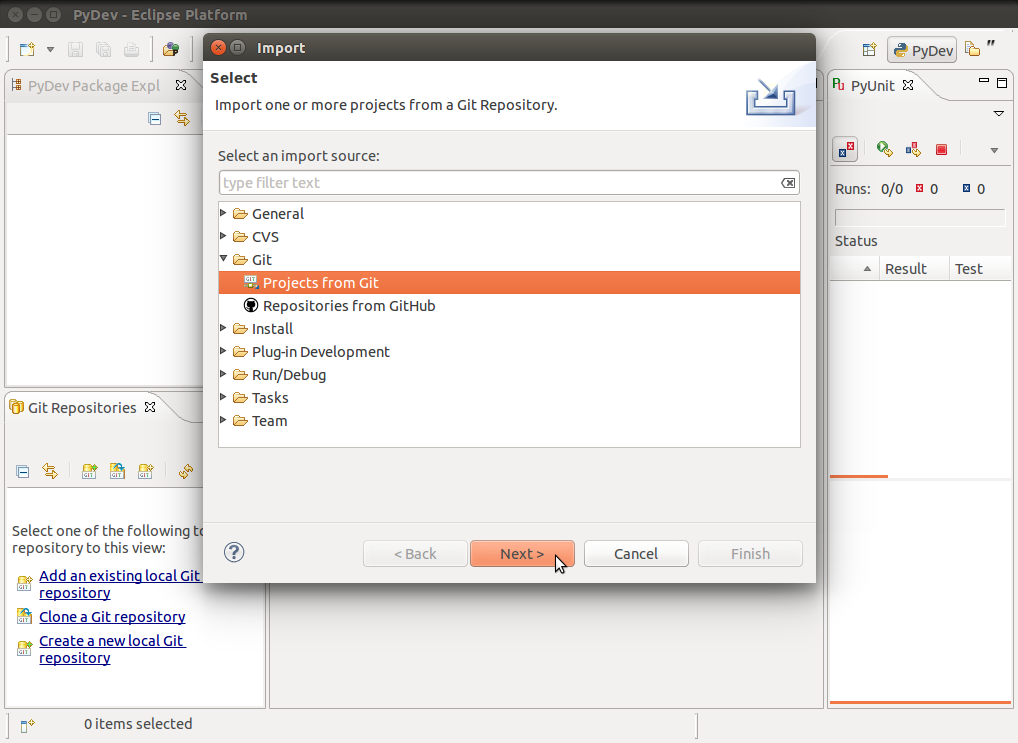
\includegraphics[width=0.8\textwidth]{images/manualtecnico/import_project01.png}
\caption{Importación do repositorio en Eclipse, paso 1}
\label{fig:import_project01}
\end{figure}
\item Seleccionar a opción GitHub e buscar o repositorio SOS Client.
\begin{figure}[H]
\centering
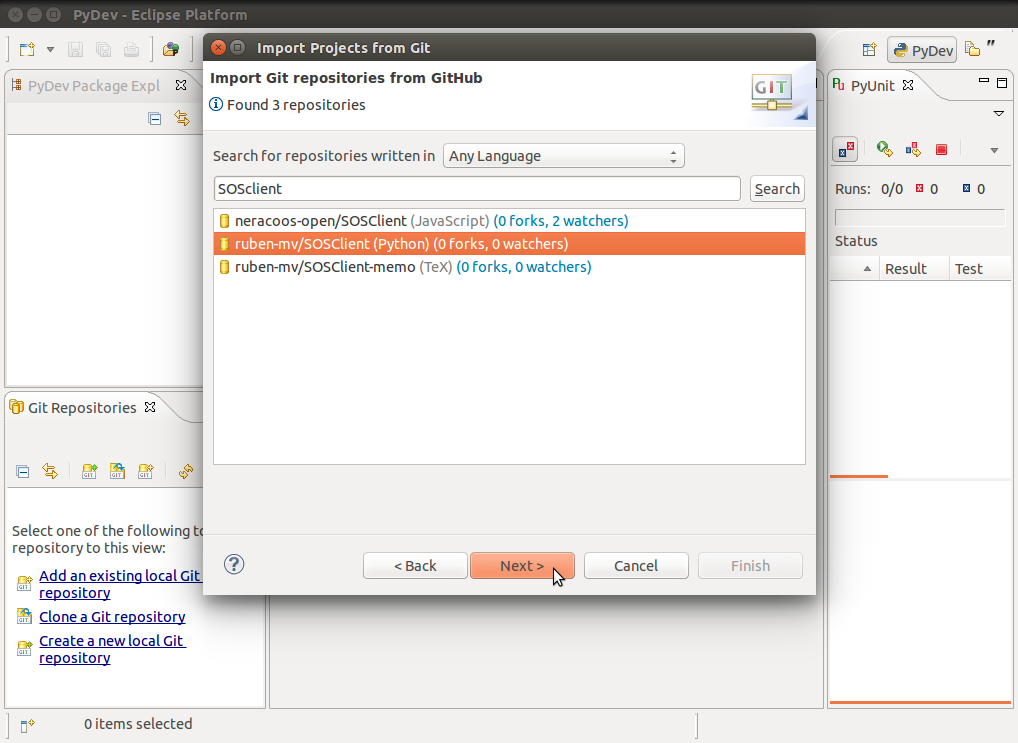
\includegraphics[width=0.8\textwidth]{images/manualtecnico/import_project02.png}
\caption{Importación do repositorio en Eclipse, paso 2}
\label{fig:import_project02}
\end{figure}
\item Engadir a rama master e importar coa opción Import as general project.
\begin{figure}[H]
\centering
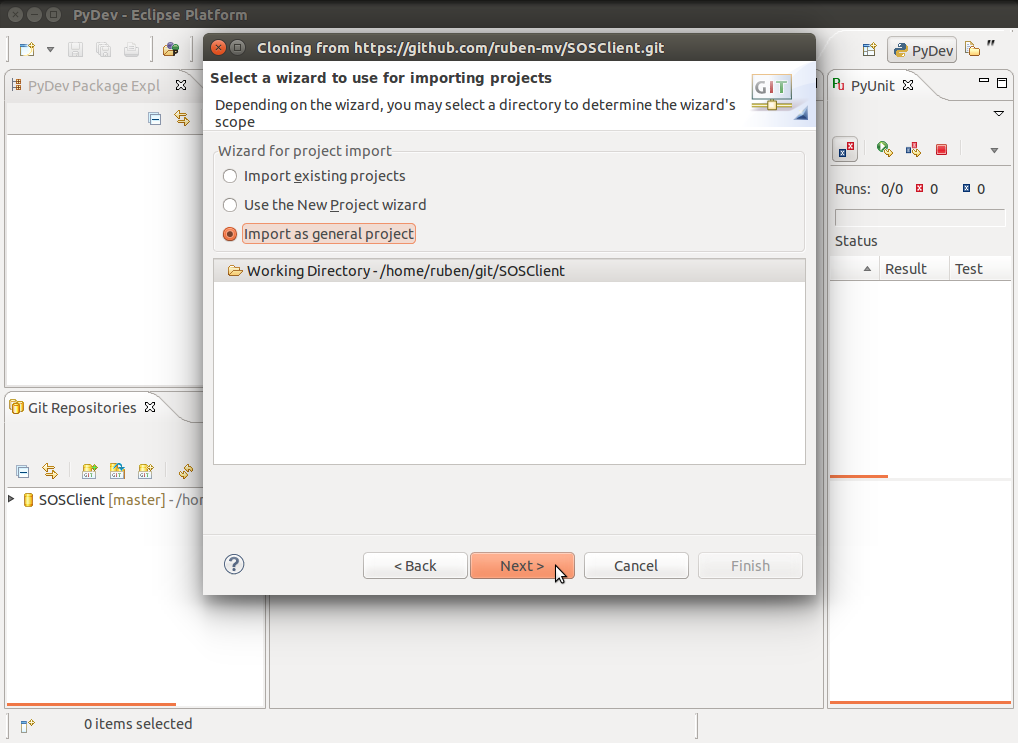
\includegraphics[width=0.8\textwidth]{images/manualtecnico/import_project03.png}
\caption{Importación do repositorio en Eclipse, paso 3}
\label{fig:import_project03}
\end{figure}
\item Unha vez feito importado o proxecto pódese converter nun proxecto de PyDev.
\begin{figure}[H]
\centering
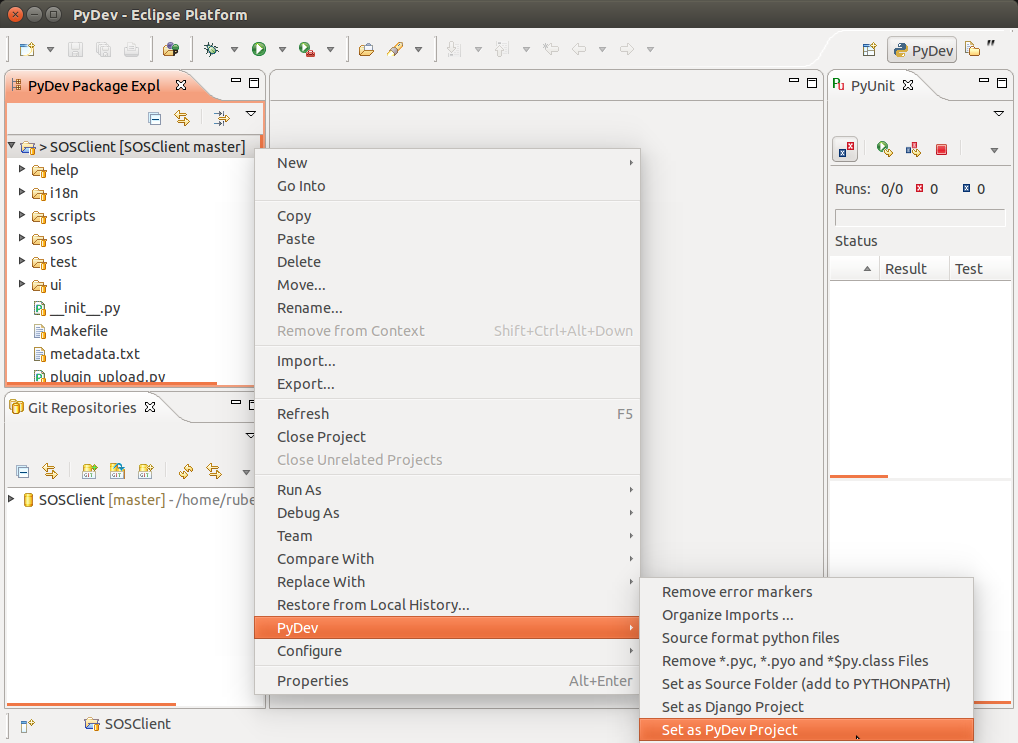
\includegraphics[width=0.8\textwidth]{images/manualtecnico/import_project04.png}
\caption{Importación do repositorio en Eclipse, paso 4}
\label{fig:import_project04}
\end{figure}
\end{itemize}

A continuación débese configurar o PyDev para que recoñeza a API de QGIS e de PyQt4 de forma que teñamos dispoñibles as funcións de autocompletado. Para esto, dende a ventá de Window $\to$ Preferences accedese á configuración do interprete de Python, onde haberá que engadir na lapela de librerías a carpeta $\sim$/.qgis/python/plugins/, e na lapela Forced builtin engadir qgis e PyQt4.
\begin{figure}[H]
\centering
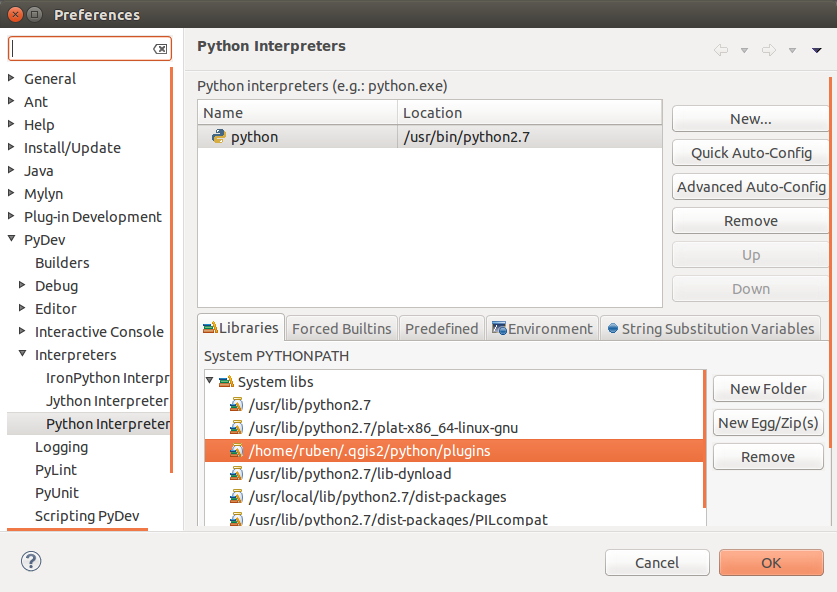
\includegraphics[width=0.75\textwidth]{images/manualtecnico/python_settings.png}
\caption{Configuración de Python en Eclipse}
\label{fig:python_settings}
\end{figure}

Tamén se deben engadir as carpetas do proxecto ó PYTHONPATH, desde as propiedades do proxecto:
\begin{figure}[H]
\centering
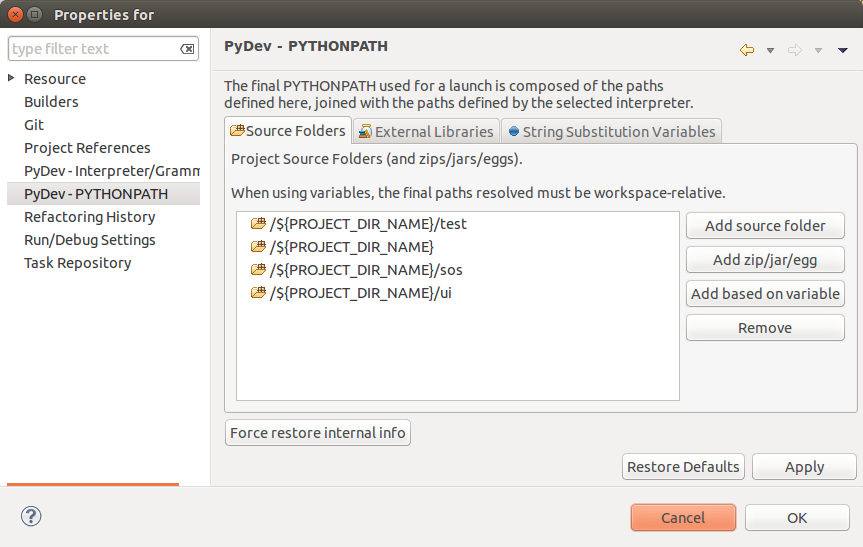
\includegraphics[width=0.75\textwidth]{images/manualtecnico/python_path.png}
\caption{Configuración do PYTHONPATH}
\label{fig:python_path}
\end{figure}


O proxecto foi creado inicialmente co plugin 'Plugin Builder'\footnote{\url{http://g-sherman.github.io/Qgis-Plugin-Builder/}} de QGIS polo que contén un Makefile que nos permite usar make coas seguintes opcións, entre outras:
\begin{description}
\item[deploy:] Desprega o plugin na carpeta correspondente.
\item[derase:] Elimina a carpeta de despregue do plugin.
\item[transup:] Actualiza os ficheiros de traducións.
\item[zip:] Desprega o plugin e crea un zip axeitado para subir ó repositorio de QGIS.
\item[test:] Executa os tests.
\end{description}

Tamén é de moita utilidade instalar no QGIS o plugin 'Plugin Reloader'\footnote{\url{http://plugins.qgis.org/plugins/plugin_reloader/}}, que se pode instalar dende o propio menú do QGIS. Este plugin permite volver a cargar un plugin dende disco sen necesidade de cerrar e volver a abrir o QGIS.

Outras ferramentas que se poden necesitar para o desenvolvemento do plugin son o QtDesigner, para modificar os ficheiros de extensión .ui nos que se define a interface gráfica, e o QtLingüist, para as traducións a distintos idiomas.

\section{Ampliación do módulo de procesamento XML}
Co obxectivo de que o módulo de procesamento se poda ampliar para dar cobertura a máis implementacións do servizo SOS e do estándar O\&M este foi deseñado de forma modular, con distintas clases específicas para o procesamento de cada parte do XML. Para engadir soporte para etiquetas xml non soportadas será necesario crear unha clase que herde de XMLParser co nome da etiqueta que procesa co sufixo Parser, de xeito que poda ser instanciada a través da factoría XMLParserFactory cando sexa necesaria.

A clase XMLParser descríbese na figura \ref{fig:xmlparser}, e forma parte do módulo xmlparser no paquete sos.

\begin{figure}[H]
\centering
\begin{minted}[framesep=2mm,bgcolor=gray!20,fontsize=\footnotesize]{python}
class XMLParser (object):
    """
    XML parser base class
    """
    __metadata__ = abc.ABCMeta

    @abc.abstractmethod
    def parse (self, xml=None):
        """
        :param xml: XML to parse
        :type xml: QDomElement or str
        """
    
    @staticmethod
    def searchFirst (xml, query):
        """
        :param xml: XML to parse
        :type xml: QDomNode
        :param query: 
        :type query: str
        :return: QDomNode, str
        """

    @staticmethod
    def search (xml, query):
        """
        :param xml: XML to parse
        :type xml: QDomNode
        :param query: 
        :type query: str
        :return: (QDomNode, str) generator
        """
\end{minted}
\caption{Definición da clase XMLParser}
\label{fig:xmlparser} 
\end{figure}

Esta clase consta de tres métodos. O método \emph{parse} é o que debe ser sobreescrito polas clases fillas, para levar a cabo as operacións que corresponda, e os métodos \emph{searchFirst} e \emph{search} están definidos para abstraer o procesamento do XML das librerías empregadas. Ambas funcións reciben como parámetro o xml sobre o que traballar e a consulta a executar, coa diferencia de que a primeira devolve a primeira ocorrencia, e a segunda permite iterar sobre todas as ocorrencias. O parámetro query permite interrogar por etiquetas, atributos, e atributos con un valor concreto. Por exemplo:

%Configuración para codigo de Python inline
\definecolor{Code}{rgb}{0,0,0}
\definecolor{Decorators}{rgb}{0.5,0.5,0.5}
\definecolor{Numbers}{rgb}{0.5,0,0}
\definecolor{MatchingBrackets}{rgb}{0.25,0.5,0.5}
\definecolor{Keywords}{rgb}{0,0,1}
\definecolor{self}{rgb}{0,0,0}
\definecolor{Strings}{rgb}{0,0.63,0}
\definecolor{Comments}{rgb}{0,0.63,1}
\definecolor{Backquotes}{rgb}{0,0,0}
\definecolor{Classname}{rgb}{0,0,0}
\definecolor{FunctionName}{rgb}{0,0,0}
\definecolor{Operators}{rgb}{0,0,0}
\definecolor{Background}{rgb}{0.98,0.98,0.98}
\lstset{
showspaces=false,
showtabs=false,
showstringspaces=false,
frame=l,
tabsize=4,
% Basic
basicstyle=\ttfamily\small,
backgroundcolor=\color{Background},
language=Python,
% Comments
commentstyle=\color{Comments}\slshape,
% Strings
stringstyle=\color{Strings},
morecomment=[s][\color{Strings}]{"""}{"""},
morecomment=[s][\color{Strings}]{'''}{'''},
% keywords
morekeywords={import,from,class,def,for,while,if,is,in,elif,else,not,and,or,print,break,continue,return,True,False,None,access,as,,del,except,exec,finally,global,import,lambda,pass,print,raise,try,assert},
keywordstyle={\color{Keywords}\bfseries},
% additional keywords
morekeywords={[2]@invariant},
keywordstyle={[2]\color{Decorators}\slshape},
emph={self},
emphstyle={\color{self}\slshape},
}
%Fin de configuración para código Python inline
\begin{itemize}
\item \lstinline|node, version = self.searchFirst (xml, "@version")|\\Devolve o atributo version da etiqueta en curso.
\item \lstinline|for _, value in self.search (xml, "resultModel"): pass|\\Itera sobre todas as etiquetas resultModel fillas do nodo xml.
\item \lstinline|for _, value in self.search (xml, "observedProperty@href"): pass|\\Itera sobre o atributo href de todas as etiquetas observedProperty fillas do nodo xml.
\item \lstinline|for node, tag in self.search (member, "Observation/*"): pass|\\Itera sobre todas as etiquetas fillas de todas as etiquetas Observation fillas do nodo xml.
\item \lstinline|opNode, _ = self.searchFirst (xml, "Operation@name=GetCapabilities")|\\Devolve o primeiro nodo de etiqueta Operation cuxo atributo name vale GetCapabilites.
\end{itemize}

